

\documentclass[aspectratio=169, 12pt]{beamer}

%%%%%%%%%%%%
% Packages %
%%%%%%%%%%%%

\usepackage{ctex}
\usepackage[english]{babel}
\usepackage{packages/sleek}
\usepackage{packages/tweaks}
\usepackage{calligra} % thanks pakeage
\usepackage{graphicx}

%%%%%%%%%%%%%%%%
% Bibliography %
%%%%%%%%%%%%%%%%

\addbibresource{./resources/bib/references.bib}

%%%%%%%%%%%%%%
% Title-page %
%%%%%%%%%%%%%%


\title{公共经济学}
\subtitle{Public Economics}
\author[LIU ShHUAI]{刘 {  } 帅}
\institute{山西师范大学 {  } 经济与管理学院}
\date{\today}
\titlelogo{./resources/pdf/logo.png}
\framelogo{./resources/pdf/logo.png}

%%%%%%%%%%%%
% Document %
%%%%%%%%%%%%

\begin{document}

\maketitle

\begin{frame}[plain]
    \frametitle{重点问题}
    \begin{itemize}
        \item \textbf{如何进行经济学研究?}
        \item \textbf{经济学研究的范式是什么?}
        \item \textbf{一篇经济学论文应该包含哪些内容?}
        \item \textbf{怎样高效地完成一篇学位论文写作?}
    \end{itemize}
\end{frame}

\begin{frame}[standout]
    第一章\par
    \addtolength{\parskip}{.4em}
    现代经济学研究框架与方法论
\end{frame}

\begin{frame}[plain]
    % \begin{multicols}{1}
    %   \frametitle{Outline}
    %   \tableofcontents[hideallsubsections]
    % \end{multicols}
    \frametitle{Outline}
    \tableofcontents[hideallsubsections]
    % \tableofcontents[currentsection]
  \end{frame}

\section{一、数据与经验典型特征事实}

\begin{frame}[plain]
    \frametitle{测度与数据收集}
    \begin{block}{测度}
        明确概念,确定基准(\emph{Benchmark},\textbf{最理想的测度数据})
    \end{block}
    \begin{block}{数据收集}
        结构数据(tabular data)、非结构数据(文本,音视频等)\par
        \addtolength{\parskip}{.8em}
        \begin{enumerate}
            \item  \textbf{调查问卷}
            \item  \textbf{田野调查}
            \item  \textbf{经济实验}
            \item  \textbf{互联网大数据}
            \item  \textbf{二手数据:统计年鉴、商业和非商业数据库}
        \end{enumerate}
    \end{block}
\end{frame}

\begin{frame}[plain]
    \frametitle{经验典型特征事实}
    经验典型特征事实(empirical stylize fact)是经济研究的出发点和基础。\par
    \textbf{可观察性、代表性、重要性、客观性} \par
    \addtolength{\parskip}{.8em}
    \begin{enumerate}
        \item  \textbf{对比-差异-分布}
        \item  \textbf{相关关系(线性、半弹性,弹性)}
        \item  \textbf{动态发展}
        \item  \textbf{已有现象的新特征}
        \item  \textbf{借助其他复杂全面的分析工具}
        \item  \ldots\ldots
    \end{enumerate}
\end{frame}

\begin{frame}[plain]
    \frametitle{经验典型特征事实--举例}
    \begin{figure}
        \centering
        \begin{minipage}[t]{0.5\linewidth}
            \centering
            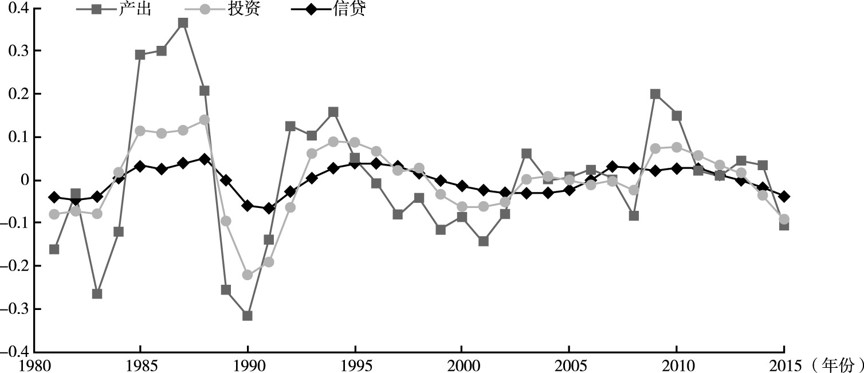
\includegraphics[width=1.0\textwidth]{./resources/figure/ecoperiod.jpg}
            \caption{经济周期}
            \label{fig:ver_2figs_2cap_1}
        \end{minipage}%
        \begin{minipage}[t]{0.5\linewidth}
            \centering
            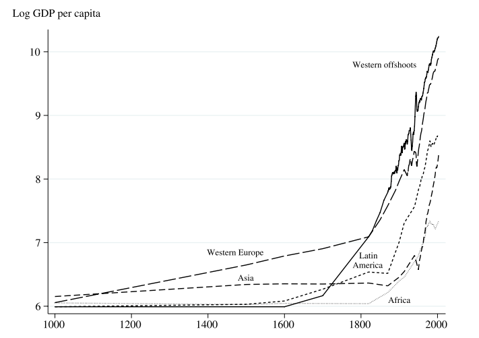
\includegraphics[width=1.0\textwidth]{./resources/figure/growth.png}
            \caption{现代经济增长}
            \label{fig:ver_2figs_2cap_2}
        \end{minipage}
    \end{figure}
\end{frame}

\section{二、理论模型构建与分析}

\begin{frame}[plain]
    \frametitle{现代经济学理论分析步骤}
    科学的经济理论分析是在概念、公理和假设基础上的逻辑推理。
    \begin{enumerate}
        \item \textbf{界定经济环境}
        \item \textbf{设定行为假设}
        \item \textbf{给出制度安排}
        \item \textbf{选择均衡结果}
        \item \textbf{评估比较}
    \end{enumerate}
    \blindfootnote{田国强.现代经济学的基本分析框架与研究方法.经济研究.2005年第2期.}
    \blindfootnote{ }
    \blindfootnote{ }
\end{frame}

\begin{frame}[plain]
    \frametitle{现代经济学分析基础}
    \textbf{经济语言}
    \par
    \textbf{数学语言(微积分,集合论,动态规划)}
    \par
    \textbf{研究平台:已有基础理论}
    \par
    \textbf{参照系:参照系指的是理想状态下的标准经济学模型, 它导致了理想的结果, 如资源有效配置等。}
\end{frame}

\section{三、实证检验分析}

\begin{frame}[plain]
    \frametitle{实证分析两大流派}
    现代经济实证分析主要有两大流派
    \begin{block}{简约式(reduced-form)}
        主要工具为计量经济学和线性代数,分析简便,假设条件较少,卢卡斯批判(预期会影响模型参数发生变化,简约式无法处理)。
    \end{block}
    \begin{block}{结构式(structure-form)}
        主要工具为计量经济学、优化理论、数值计算、线性代数,可进行反事实分析,假设条件较多,主要基于模拟分析。
    \end{block}
    \blindfootnote{科学研究主要采用排除法,尤其是在社会科学研究,只可以证伪}
    \blindfootnote{ }
    \blindfootnote{ }
\end{frame}

\section{四、实践应用}

\begin{frame}[plain]
    \frametitle{实践应用} 
    \begin{enumerate}
        \item \textbf{现象解释}
        \item \textbf{未来预测}
        \item \textbf{政策干预}
        \item \textbf{政策评估}
    \end{enumerate}
\end{frame}

\section{五、文献研究}

\begin{frame}[plain]
    \frametitle{文献检索、管理与阅读}
    文献检索:知网, web of science,NBER(working paper),ReasearchRabbit,Paper Digest。
    \par
    检索关键词1-2个,注意同义词变换。
    \par
    文献下载:SCI-HUB,知网,谷歌学术,百度学术。
    \par
    文献管理软件:Endnote(商业)、Mendeley(开源)、Zotero(开源)、NoteExpress(商业)、Citavi(商业)
    \par
    文献阅读:速读或者精度,找出文献所研究的经验典型特征事实、理论模型、实证方法以及结论。
\end{frame}

% ---------------------------------------------------------------------------
\begin{frame}[standout]
    \begin{center}
        {\Huge\calligra Thanks!}
      \end{center}
\end{frame}
% ---------------------------------------------------------------------------

\end{document}
